\subsection{6.2 问题二模型建立与求解}

在问题二中，我们在保持问题一可行域约束不变的前提下，引入了需求、产量、成本与价格等市场与生产参数的年际波动，将其建模为随机变量，并通过多情景仿真刻画不确定性影响。首先，根据题设区间或波动范围对预期销量、亩产量、种植成本及销售价格进行采样，生成多条完整的 2024--2030 年参数路径。在每个情景下，利用超产折价销售规则计算年度总利润，并将利润不足部分定义为 Shortfall 损失 $L = \max(I - \Pi, 0)$，进一步在置信度 $\alpha=0.95$ 下计算条件在险价值 $\mathrm{CVaR}_\alpha(L)$ 作为极端风险度量。优化目标采用均值--风险权衡形式 $\max E[\Pi] - \lambda \cdot \mathrm{CVaR}_\alpha(L)$，通过遗传算法在多情景利润分布下迭代寻优，得到兼顾收益与稳健性的种植方案，并输出期望利润与风险指标，用于构建风险--收益前沿与年度面积配置方案。

\begin{figure}[H]
    \centering
    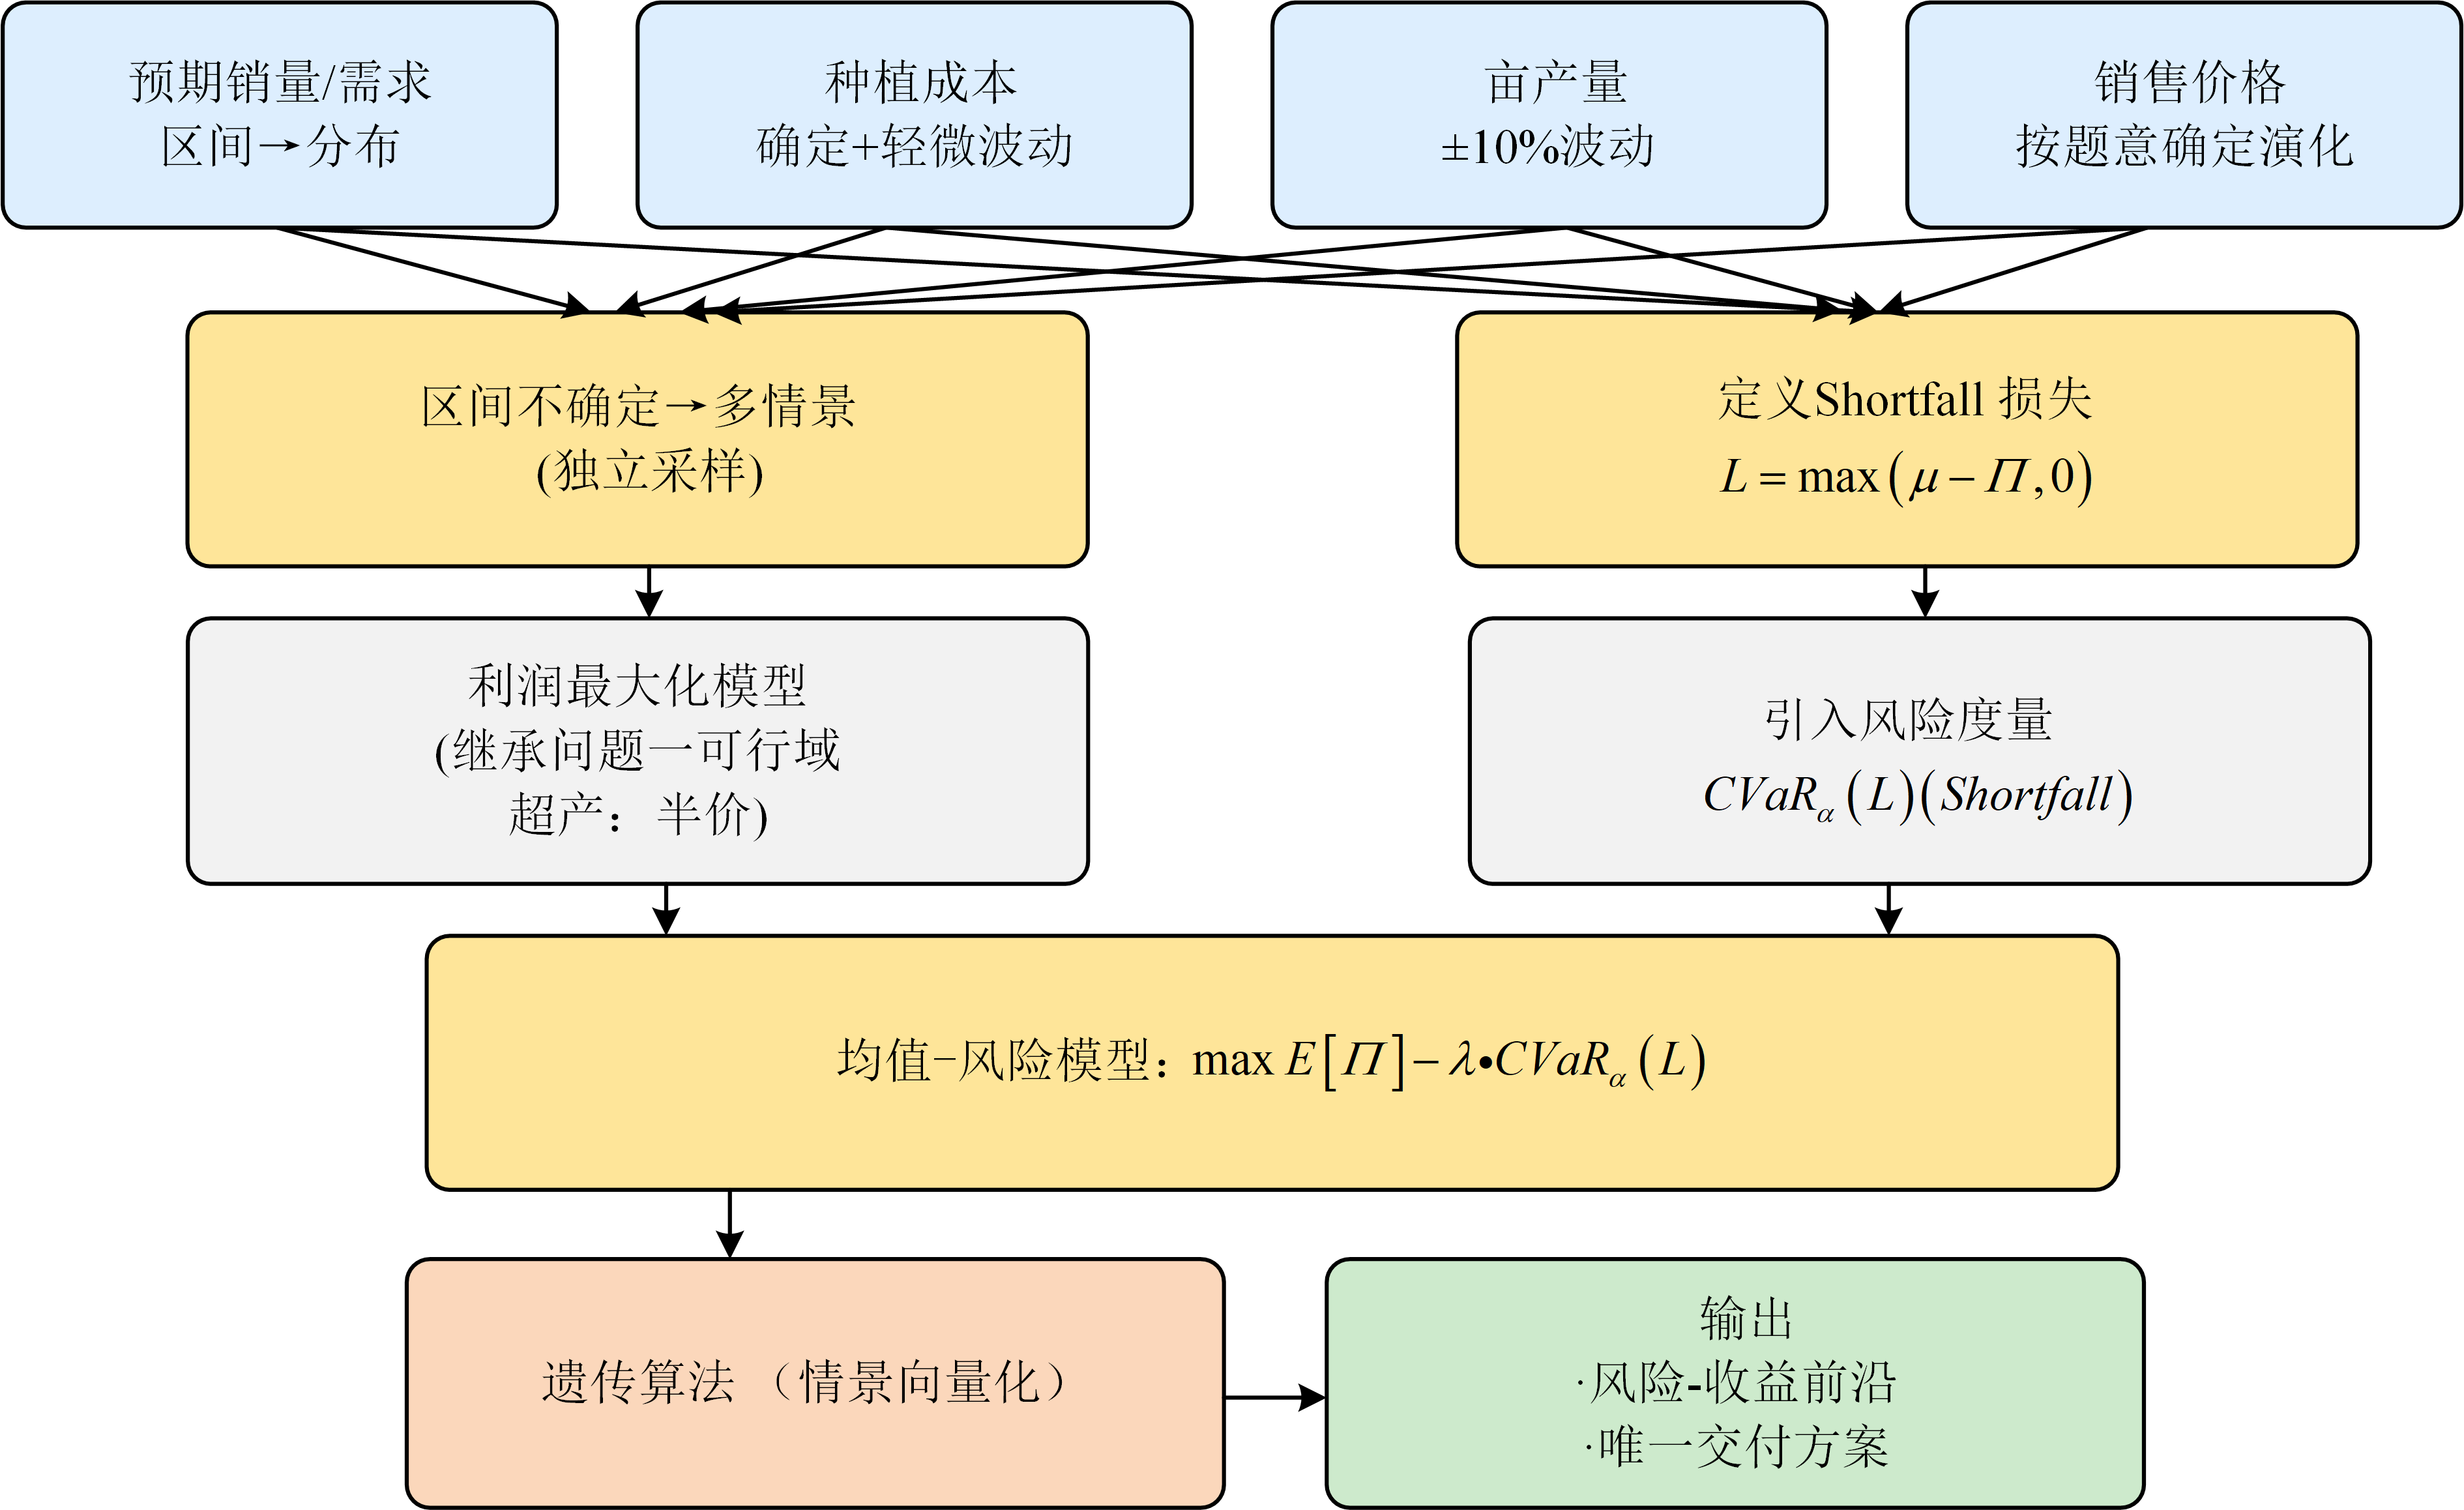
\includegraphics[width=0.8\textwidth]{mindmap/pb2.png} % 耕地类型占比图
    \caption{问题二求解流程图}
    \label{fig:mmp_pb2}
\end{figure}
在问题二中，我们在保留问题一可行域约束（地块适宜性、轮作重茬、三年豆类覆盖率、作物分散度等）的基础上，仅将赛题中给出具有区间波动或年变化趋势的参数建模为随机变量，其余参数保持为确定值，具体处理方式如下：
小麦与玉米年增长率 $g_{wc} \sim U(0.05, 0.10)$，即 $D_{c,y} = D_{c,2023} \cdot (1+g_{wc})^{y-2023}$；其他作物年变动率 $\epsilon \sim U(-0.05, 0.05)$，即 $D_{c,y} = D_{c,2023} \cdot (1+\epsilon)$。
亩产量年波动率 $\delta \sim U(-0.10, 0.10)$，则 $q_{c,y} = q_{c,2023} \cdot (1+\delta)$。
种植成本年通胀率 $r_{\text{inf}} \sim U(0.03, 0.07)$，成本随年份累积增长，即 $k_{c,y} = k_{c,2023} \cdot \prod_{\tau=2024}^{y} (1+r_{\text{inf},\tau})$。
对于销售价格, 粮食类作物价格稳定，$p_{c,y} = p_{c,2023}$；蔬菜类作物：设年增长率为 $5\%$，即 $p_{c,y} = p_{c,2023} \cdot 1.05^{y-2023}$；食用菌类作物年下降率 $r_{\text{fungi}} \sim U(0.01,0.05)$，即 $p_{c,y} = p_{c,2023} \cdot \prod_{\tau=2024}^{y} (1-r_{\text{fungi},\tau})$；其中羊肚菌固定下降 $5\%$/年。
以上随机变量在多情景仿真中独立采样生成，形成2024--2030 年的完整参数路径。超额产出按当年售价的 $50\%$ 折价销售。

\subsection{6.2.1 决策变量}
决策采用地块—年—季—作物四维 0-1 变量
\[
z_{\ell y s c}\in\{0,1\},\qquad (\ell\in\mathcal L,\ y\in\mathcal Y,\ s\in\mathcal S,\ c\in\mathcal C),
\]
表示是否在 $(\ell,y,s)$ 种植作物 $c$。实现中以\emph{整数基因编码}并在解码时用\emph{可行性掩码}过滤不适宜的地块类型—季别—作物组合。
\subsection{6.2.2 收益、成本与风险口径}
在场景 $\omega$、年份 $y$ 下，作物 $c$ 的产量与收入为
\[
P_{c,y}=\sum_{\ell\in\mathcal L}\sum_{s\in\mathcal S} a_{\ell s}\, q_{c,y}^{(\omega)}\, z_{\ell y s c},\qquad
R_{c,y}^{(\omega)}=p_{c,y}^{(\omega)}\!\cdot\!\min\!\{P_{c,y},D_{c,y}^{(\omega)}\}+0.5\,p_{c,y}^{(\omega)}\!\cdot\!\max\!\{0,P_{c,y}-D_{c,y}^{(\omega)}\}.
\]
对应的成本
\[
C_{y}^{(\omega)}=\sum_{\ell,s,c} a_{\ell s}\,k_{c,y}^{(\omega)}\,z_{\ell y s c},\qquad
\Pi^{(\omega)}=\sum_{y,c} R_{c,y}^{(\omega)}- \sum_y C_{y}^{(\omega)}.
\]
为抑制尾部亏损，采用\textbf{条件在险价值}（CVaR）约束目标。设置信度 $\alpha=0.95$，记损失 $L^{(\omega)}=-\Pi^{(\omega)}$，则
\[
\text{CVaR}_\alpha(L)=\mathbb{E}\!\left[L^{(\omega)}\mid L^{(\omega)}\ge \text{VaR}_\alpha(L)\right].
\]
问题二的\emph{风险—收益权衡}目标为
\[
\max\ \ \mathbb{E}_\omega[\Pi^{(\omega)}]\ -\ \lambda\cdot \text{CVaR}_{0.95}\!\big(L^{(\omega)}\big),
\]
其中 $\lambda$ 为权重（默认 $\lambda=0.10$）。实现中以\emph{样本平均}估计 $\mathbb{E}[\cdot]$，并以\emph{分位截尾均值}估计 CVaR。

\subsection{6.2.3 问题二求解过程：情景—遗传算法（Scenario--GA）} 
\noindent \textbf{场景生成} 按设定随机生成 $N=300$ 条 2024--2030 的参数路径（需求、亩产、价格、成本）并缓存为张量 \texttt{DEMAND}, \texttt{YIELD}, \texttt{PRICE}, \texttt{COST}; \\
\textbf{编码与解码} 个体长度 $|\mathcal L|\times|\mathcal Y|\times 2$（两季），整数基因 $\{0,\ldots,|\mathcal C|\}$；解码时应用可行性掩码 \texttt{compat} 将非法作物置零;  \\
\textbf{适应度评估} 向量化计算所有场景利润 $\Pi^{(\omega)}$，减去罚分并据此计算 $\mathbb{E}[\Pi]-\lambda\cdot \text{CVaR}_{0.95}(L)$ 作为适应度；  \\
\textbf{演化参数} 锦标赛选择、两点交叉（概率 $0.8$）、均匀变异（\texttt{indpb}$=0.03$），种群规模 $240$、迭代 $450$ 代；  \\
\textbf{结果输出} 最优个体写回 \verb|result2.xlsx|（各年工作表、两季分区，按“地块行 × 作物列”填入面积)。

\subsection{6.2.4 求解结果与可视化}
\paragraph{输出口径} 代码将 2024--2030 年的地块—作物面积矩阵写入 \verb|result2.xlsx|；同时打印\emph{经济期望利润}与\emph{CVaR95\%（亏损）}等指标，便于与不同 $\lambda$、不同场景数 $N$ 做稳健性对比。

\begin{figure}[htbp]
  \centering
  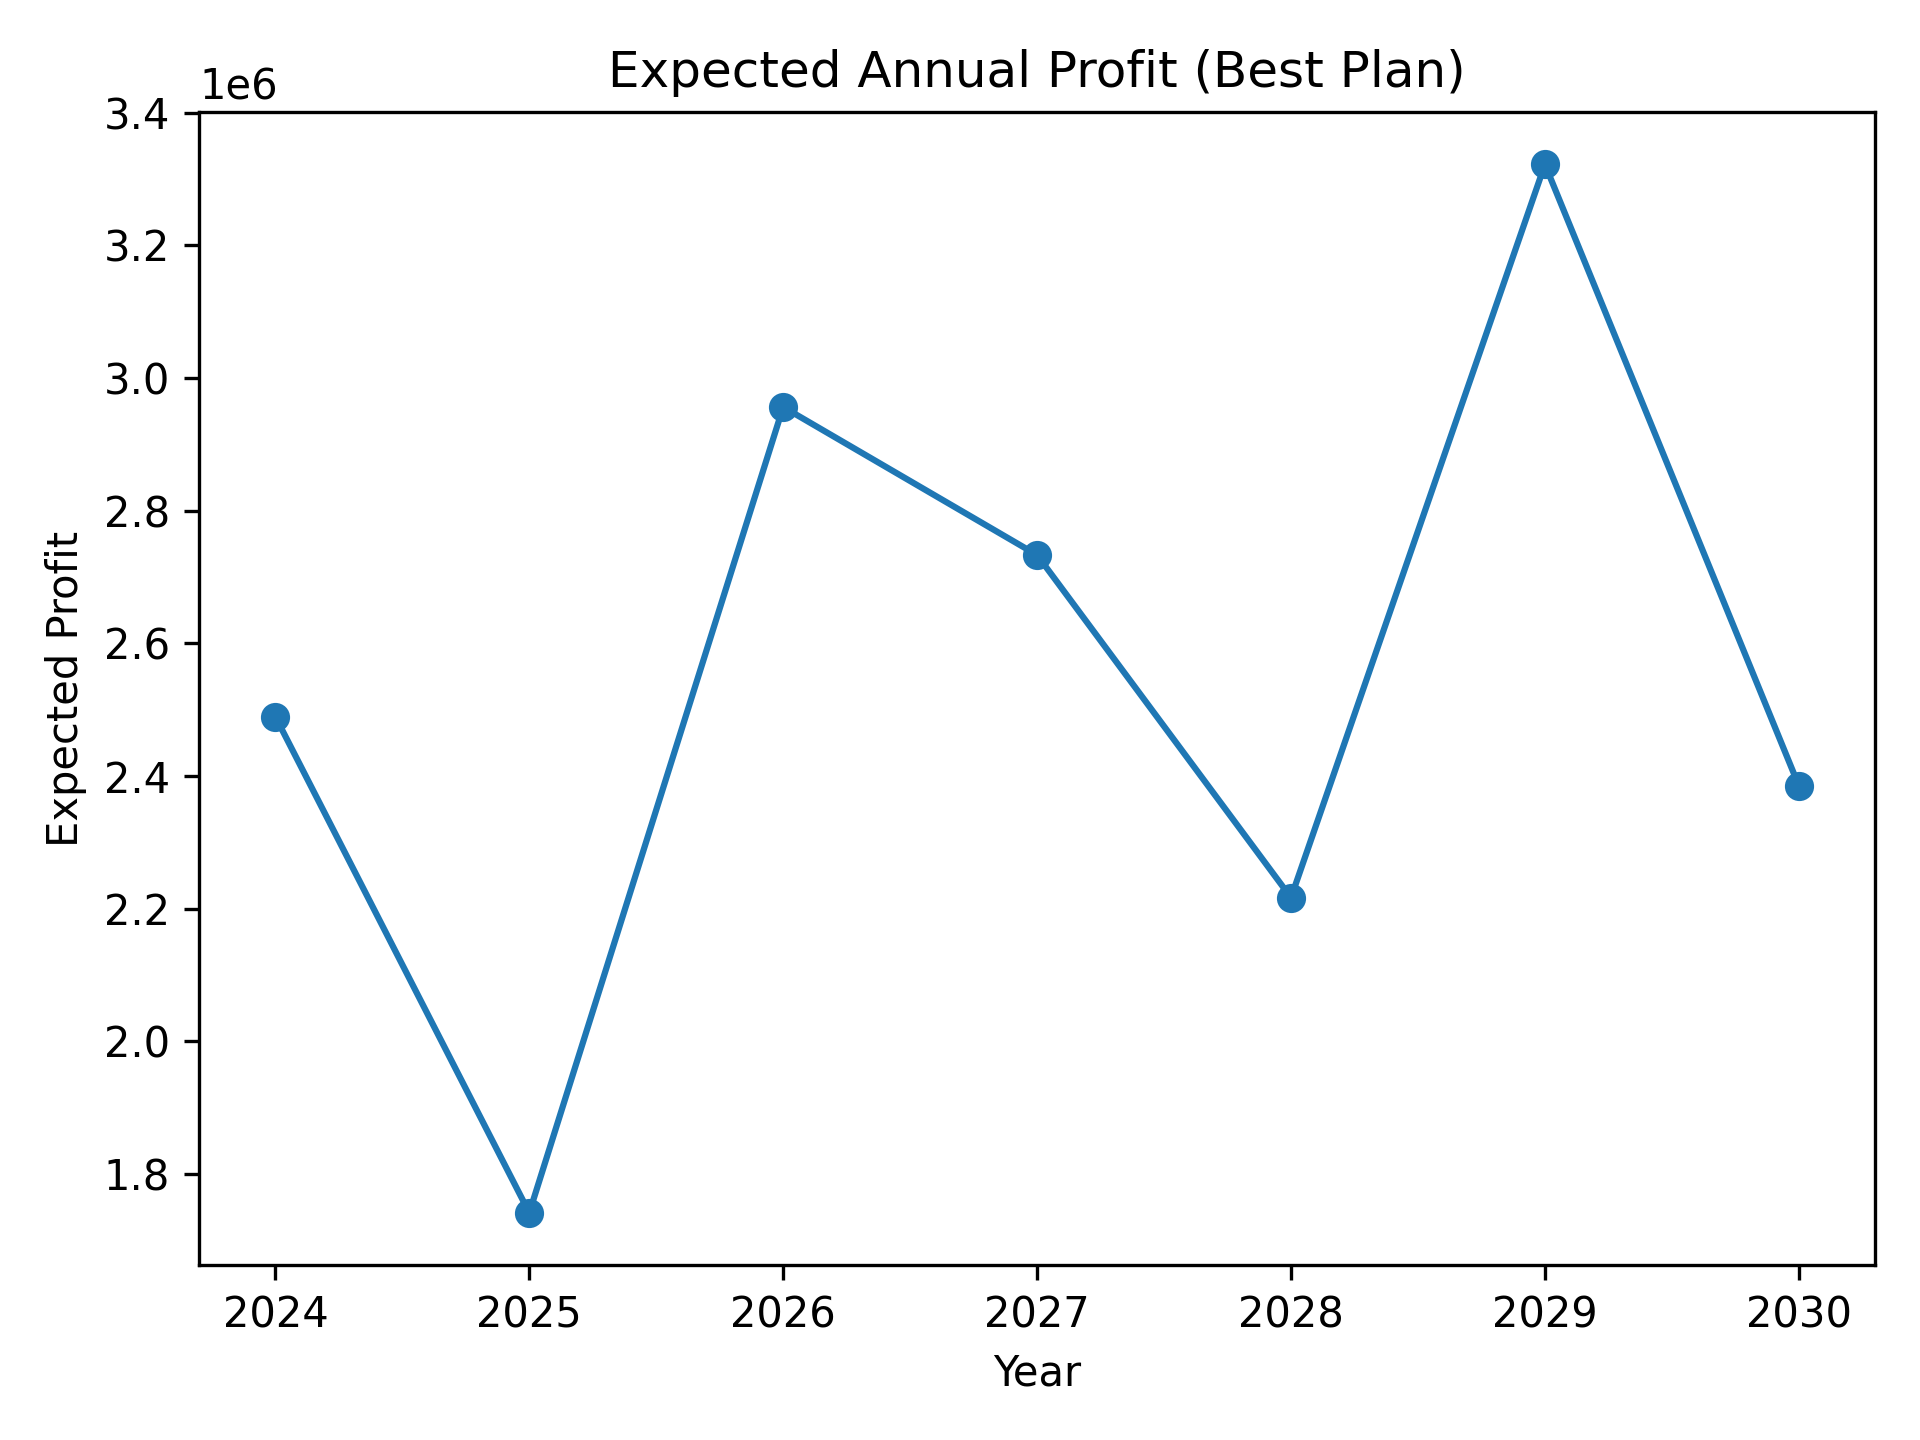
\includegraphics[width=0.85\linewidth]{figure_pb2/52bbcae1b8a57b4d8419f18e54723e59.png}
  \caption{问题二情景下最优方案的年度期望利润（2024--2030）}
  \label{fig:profit_q2}
\end{figure}

图\ref{fig:profit_q2} 展示了在考虑销量、产量、价格、成本等不确定性以及折价销售与风险惩罚后的\textbf{年度期望利润}。年度利润在不同年份间存在波动，其中 2025 年出现显著低谷，可能由不利的市场与产量情景叠加引起；,2029 年利润达到峰值，说明当年作物结构与市场条件的匹配度高,利润波动反映了模型在不同年度对高风险作物的适度回避与结构调整，这是 CVaR 风险约束作用的结果。

\begin{figure}[htbp]
  \centering
  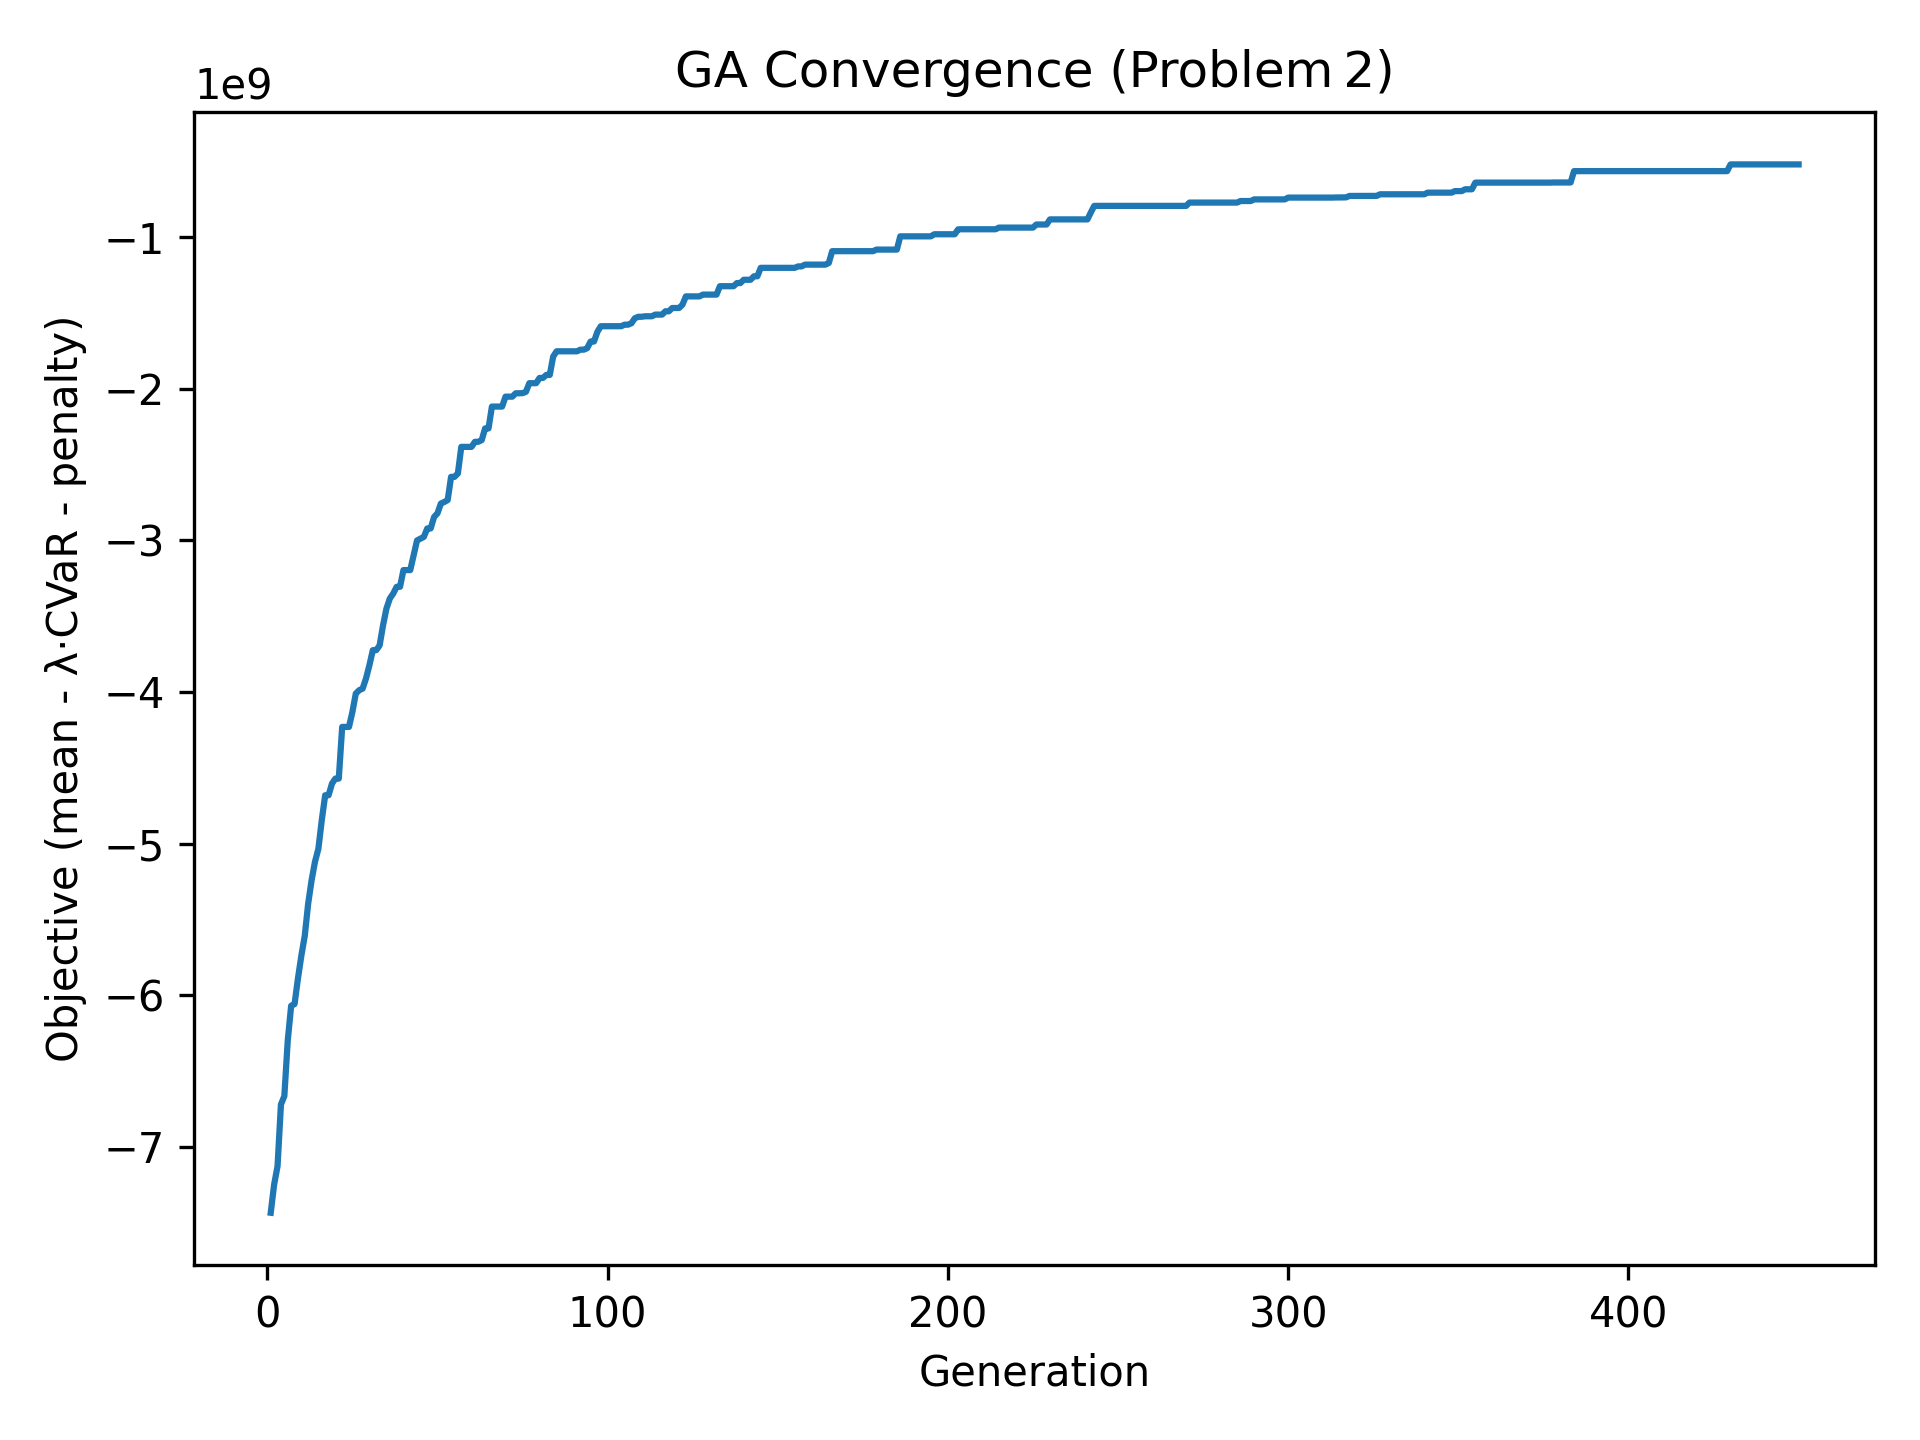
\includegraphics[width=0.85\linewidth]{figure_pb2/7a60f47d3ac8127fa0170bac7a863a80.png}
  \caption{遗传算法在问题二中的收敛过程}
  \label{fig:ga_q2}
\end{figure}

图\ref{fig:ga_q2} 显示了遗传算法在 450 代迭代中的\emph{目标值}变化情况，目标值定义为
\[
\mathbb{E}[\Pi] - \lambda\cdot\text{CVaR}_{95\%}(\text{亏损}) - \text{罚分}.
\]

优化模型的目标函数值：
\begin{equation}
\mathrm{Objective} = \mathbb{E}[\Pi(\omega)] - \lambda \cdot \mathrm{CVaR}_{0.95}(L) - \mathrm{Penalty},
\end{equation}
其中 $\mathbb{E}[\Pi(\omega)]$ 表示多情景下的平均利润，$\mathrm{CVaR}_{0.95}(L)$ 为最差 $5\%$ 场景下亏损的条件期望，$\lambda$ 为风险权重系数；Penalty 为约束罚分，包括地块适宜性、轮作重茬、三年豆类覆盖率以及作物分散度等硬性约束的惩罚项，其量级高达 $10^7$ 元。\\
优化模型的目标函数值：
\begin{equation}
\mathrm{Objective} = \mathbb{E}[\Pi(\omega)] - \lambda \cdot \mathrm{CVaR}_{0.95}(L) - \mathrm{Penalty},
\end{equation}
其中 $\mathbb{E}[\Pi(\omega)]$ 表示多情景下的平均利润，$\mathrm{CVaR}_{0.95}(L)$ 为最差 $5\%$ 场景下亏损的条件期望，$\lambda$ 为风险权重系数；Penalty 为约束罚分，包括地块适宜性、轮作重茬、三年豆类覆盖率以及作物分散度等硬性约束的惩罚项，其量级高达 $10^7$ 元。该设计旨在使严重违反约束的解在进化过程中被快速淘汰。

在演化初期，种群中大多数个体不仅经济利润较低，还存在严重的约束违反，导致罚分总额和风险惩罚项远大于利润值，从而使目标函数呈现大幅负值。随着迭代推进，遗传算法逐步修复不可行解，降低罚分并改善收益--风险平衡，目标函数值快速上升并趋于稳定。因此，纵坐标的负值仅反映了优化早期约束违反程度与风险水平较高的状态，并不意味着种植方案在经济上亏损。在演化初期，种群中大多数个体不仅经济利润较低，还存在严重的约束违反，导致罚分总额和风险惩罚项远大于利润值，从而使目标函数呈现大幅负值。随着迭代推进，遗传算法逐步修复不可行解，降低罚分并改善收益--风险平衡，目标函数值快速上升并趋于稳定。

结合两幅图可知，最终的最优种植方案在多数年份保持了较高的期望利润，并有效降低了极端亏损风险。这表明风险约束促使模型在高收益与稳健性之间取得平衡,遗传算法在此多情景、多约束的复杂组合优化中具有良好的收敛性与稳定性。

